\newpage

\section*{\centerline{Цель работы}}

Получение навыков работы с командной строкой UNIX и UNIX-подобных систем, а также навыки работы с файлами: просмотр редактирование, поиск и архивирование в GNU/Linux. Изучить основные команды и утилиты, поработать с правами на файлы и директории в GNU/LINUX. 
\newpage

\section*{\centerline{Выполнение}}
	\vspace{1cm}

	\subsection*{\centerline{Часть 1}}
		\vspace{0.5cm}
		\centerline{Цель задачи}
		1) Изучение команд для скачивания файлов из Интернета.\\
		2) Изучение команд для работы с архивами.\\
		3) Изучение команд для поиска файлов и слов в файлах.\\
		\vspace{1cm}


		\paragraph*{1.1)Скачивание файлов из интернета с использованием терминала\\\\}

		Команда \textit{wget --spider url} позволяет проверить доступность файла по указанному адресу.\\
		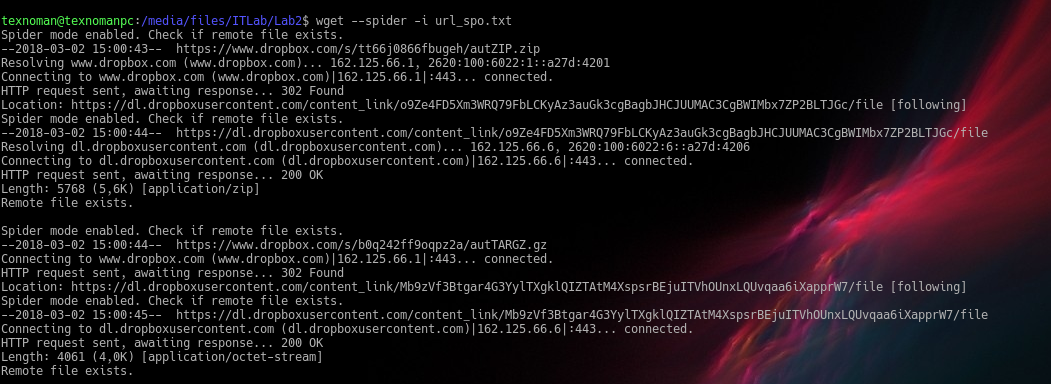
\includegraphics [width=\textwidth]{picture1.png}\\
		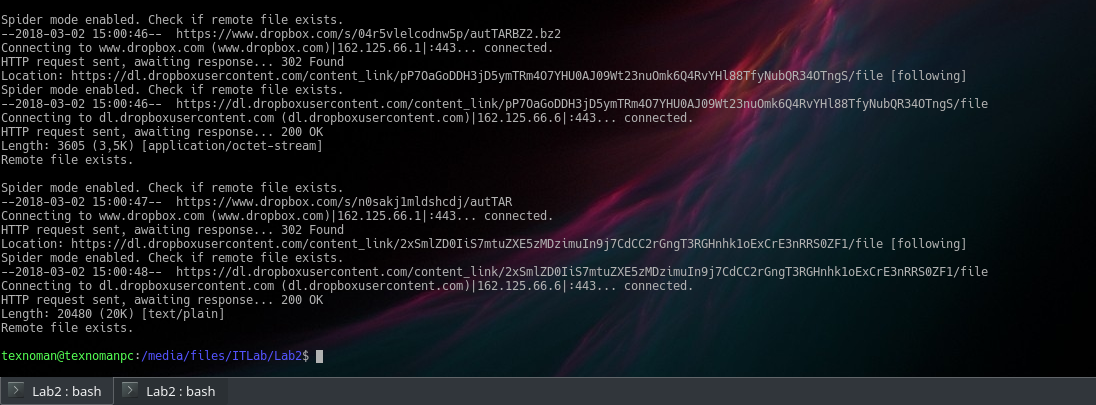
\includegraphics [width=\textwidth]{picture2.png}\\
		\vspace{0.5cm}

		Команда \textit{wget -i filename} позволяет скачать файл по ссылке из файла. С помощью \textit{head -n 1} можно получить первую строку файла\\
		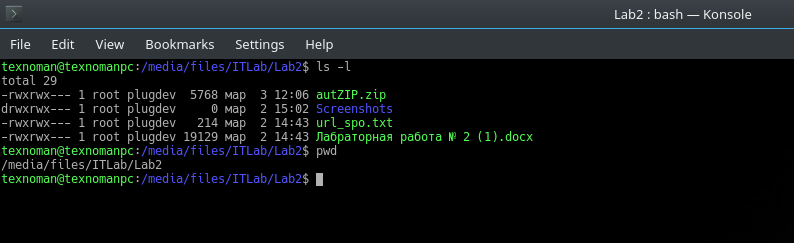
\includegraphics [width=\textwidth]{picture3.png}\\
		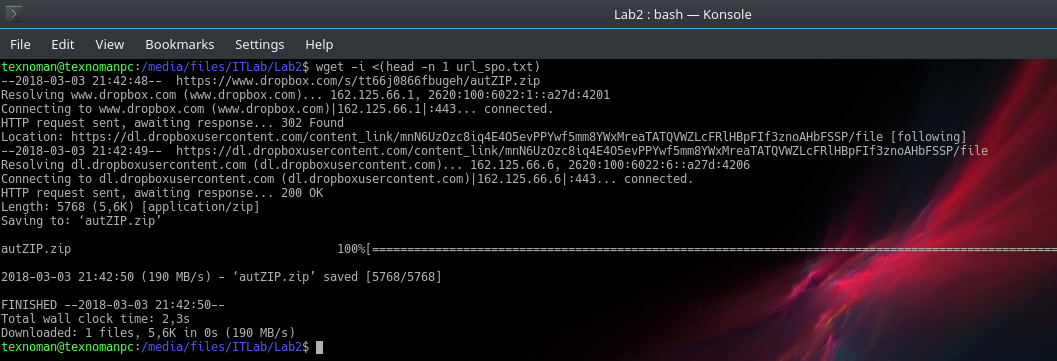
\includegraphics [width=\textwidth]{picture4.png}\\
		\vspace{0.5cm}

		Скачивание файла по второй ссылке из файла\\
		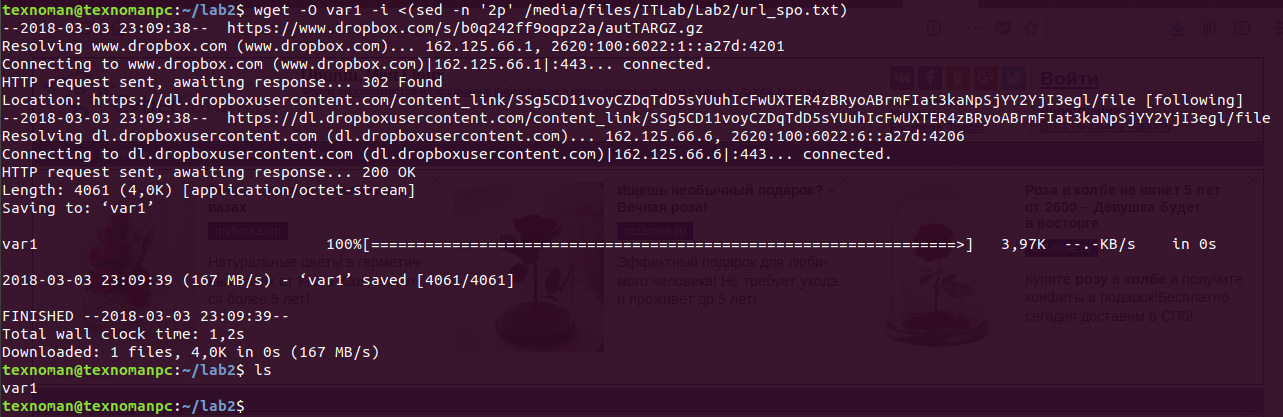
\includegraphics [width=\textwidth]{wget(var1).png}\\

		Выборку остальных файлов можно осуществить при помощи команды \textit{sed}, способной получить сразличные строки\\
		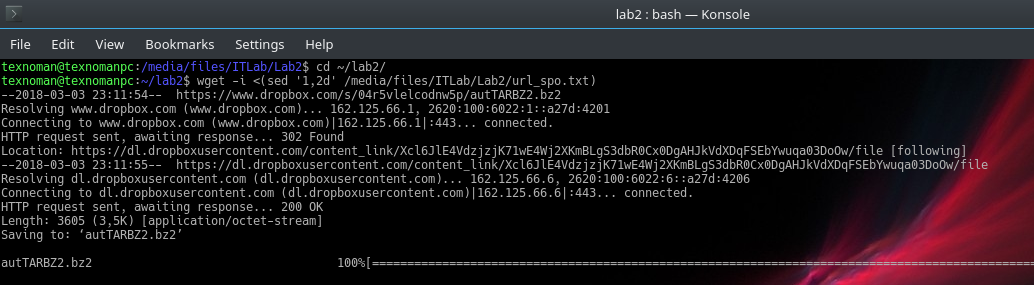
\includegraphics [width=\textwidth]{picture5.png}\\
		\vspace{0.5cm}

		Скачивание всех \textit{.jpeg}, \textit{.jpg} файлов с сайта про Лермонтова\\
		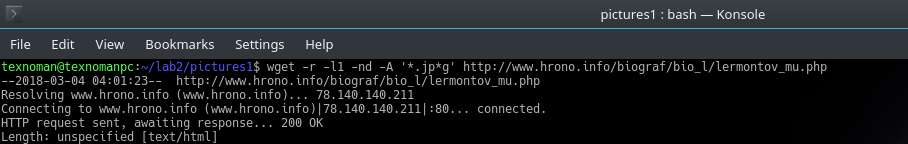
\includegraphics [width=\textwidth]{picture6.png}\\
		\vspace{1cm}
		


		\paragraph*{1.2) Работа с архивами\\\\}

		Извлечение из \textit{.zip} архива файла Лермонтов.txt\\
		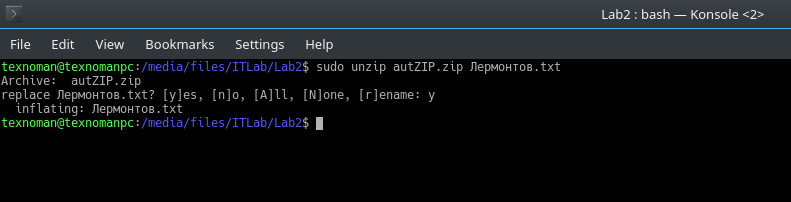
\includegraphics [width=\textwidth]{picture22.png}\\
		\vspace{0.5cm}

		Распаковка архивов \textit{.tar, .tar.gz, .tar.bz2} с выводом информации о процессе на экран\\
		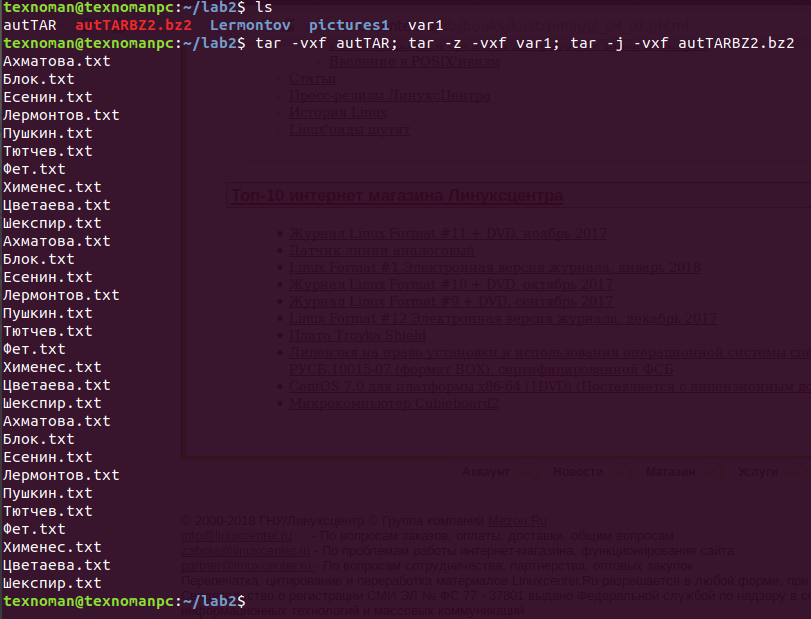
\includegraphics [width=\textwidth]{tar(3).png}\\
		\vspace{0.5cm}


		\paragraph*{1.3) Поиск файлов, поиск по тексту\\\\}
		
		Нахождение всех файлов, созданных за последний 1 дней в домашней папке\\
		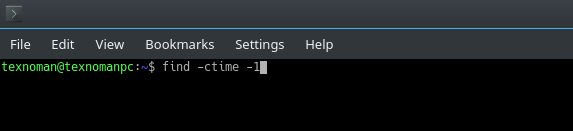
\includegraphics [width=\textwidth]{picture23.png}\\
		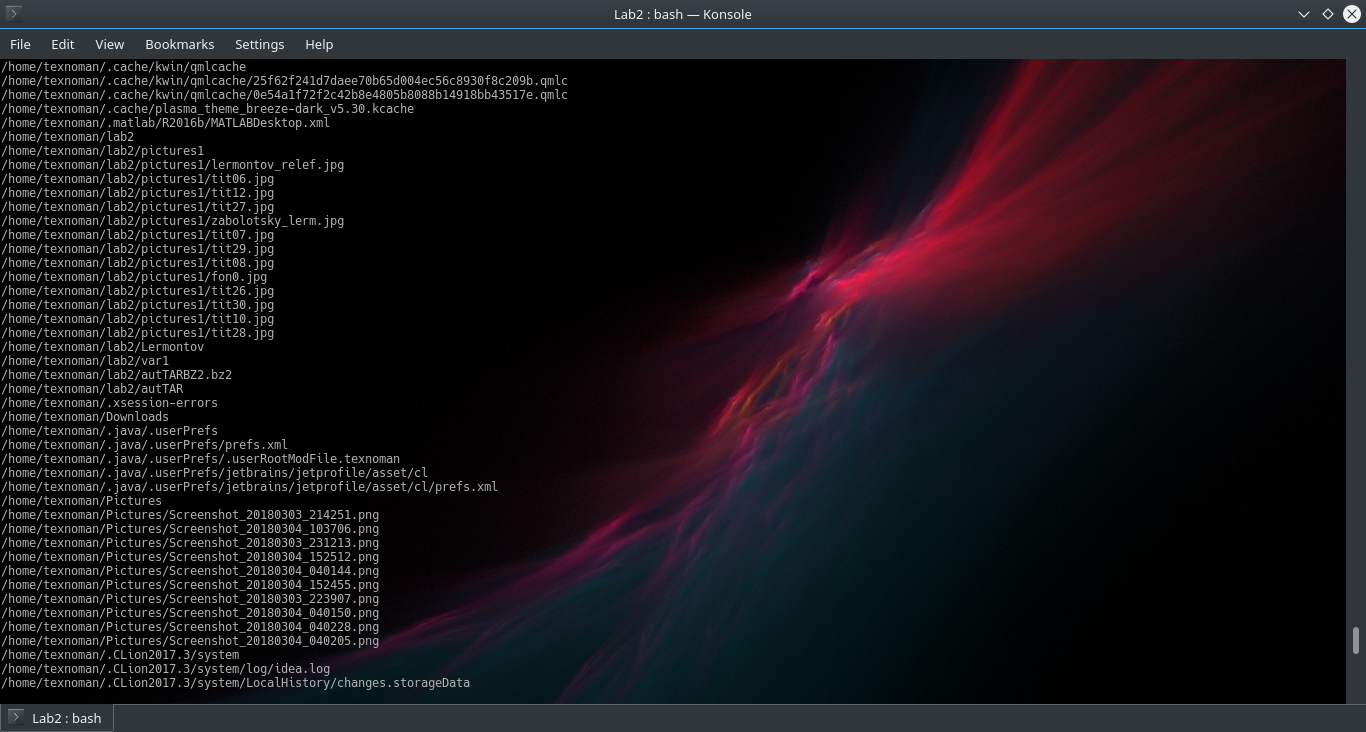
\includegraphics [width=\textwidth]{picture12.png}\\
		\vspace{0.5cm}

		Нахождение всех файлов с фамилией Лермонтов\\
		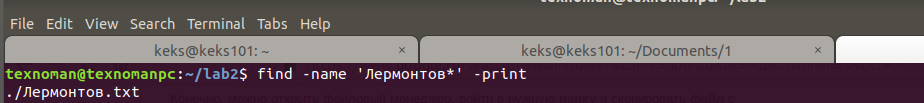
\includegraphics [width=\textwidth]{find_Lermontov.png}\\
		\vspace{0.5cm}

		Перемещение этого файла в папку \textit{Произведения Лермонтова}. Перемещение туда же файлов с картинками из сайта о Шекспире\\
		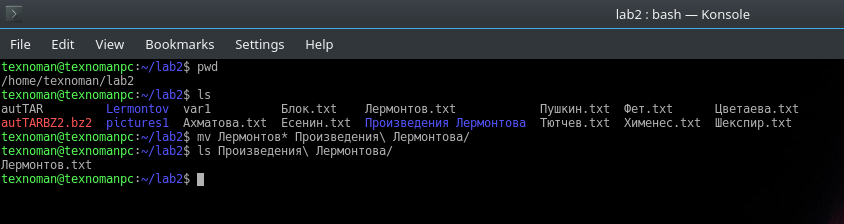
\includegraphics [width=\textwidth]{picture14.png}\\
		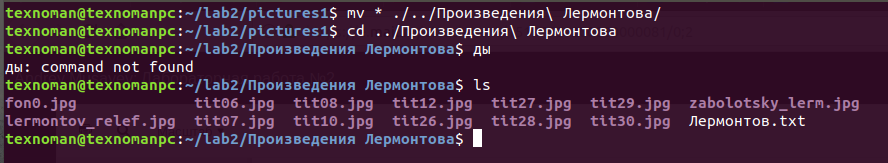
\includegraphics [width=\textwidth]{101.png}\\
		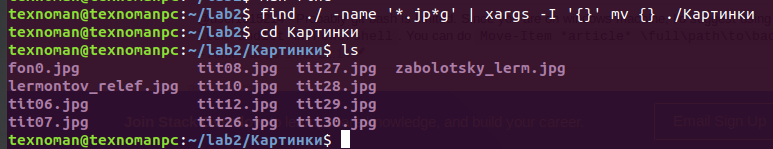
\includegraphics [width=\textwidth]{102.png}\\
		\vspace{0.5cm}

		Смена кодировки файла \textit{Лермонтов.txt} c \textit{windows-1251} на \textit{Unicode}\\
		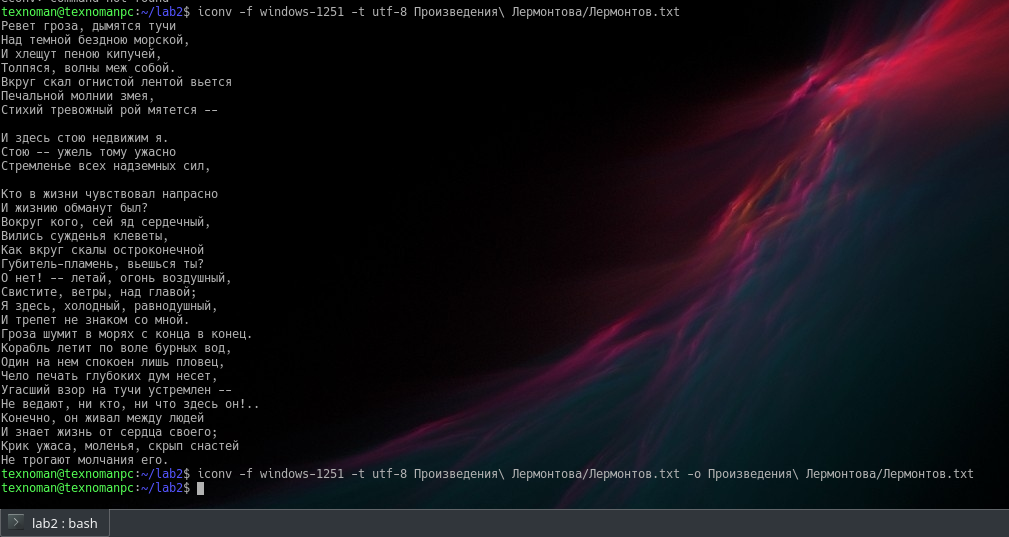
\includegraphics [width=\textwidth]{picture16.png}\\
		\vspace{0.5cm}

		Поиск слов \textit{я, то?} (\textit{?}- является спец. символом) в файле, подсчет строк может быть осуществлен при использовании ключа \textit{-c}\\
		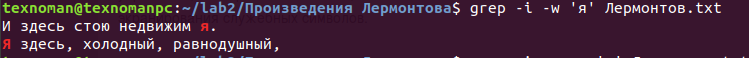
\includegraphics [width=\textwidth]{103.png}\\
		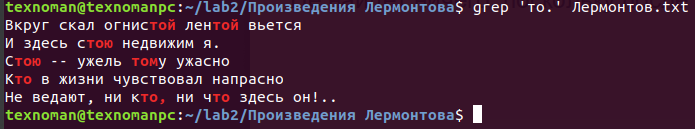
\includegraphics [width=\textwidth]{119.png}\\
		\vspace{0.5cm}

		Посчет количества строк в файлах с произведениями\\
		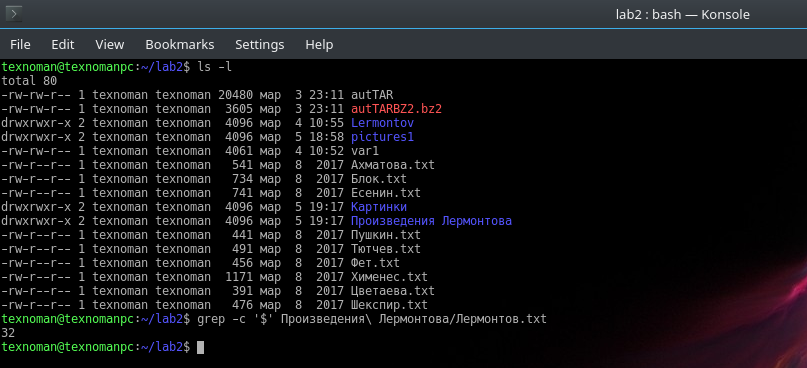
\includegraphics [width=\textwidth]{picture17.png}\\
		\vspace{0.5cm}

